% SPDX-License-Identifier: CC0-1.0
\documentclass[11pt]{article}
\usepackage[T1]{fontenc}
\usepackage[utf8]{inputenc}
\usepackage{lmodern}
\usepackage[a4paper,margin=2.35cm,headheight=14pt]{geometry}
\usepackage{amsmath,amssymb,amsthm,mathtools}
\usepackage{microtype,booktabs,array,longtable,multicol,graphicx}
\usepackage[dvipsnames]{xcolor}
\usepackage{enumitem,fancyhdr,titlesec}
\usepackage[colorlinks=true,linkcolor=MidnightBlue,citecolor=MidnightBlue,urlcolor=MidnightBlue]{hyperref}
\definecolor{Ink}{HTML}{16324F}
\definecolor{Accent}{HTML}{4E5C3D}
\titleformat{\section}{\Large\bfseries\color{Ink}}{\thesection}{.7em}{}
\titleformat{\subsection}{\large\bfseries\color{Accent}}{\thesubsection}{.7em}{}
\pagestyle{fancy}
\fancyhf{}
\fancyhead[L]{\small Two-coin entropy counterexamples}
\fancyhead[R]{\small Research draft}
\fancyfoot[C]{\thepage}
\setlength{\parskip}{.32em}
\setlength{\parindent}{1.25em}
\setlength{\emergencystretch}{2em}
\setlist{itemsep=.2em,topsep=.35em}
\numberwithin{equation}{section}
\newtheorem{theorem}{Theorem}[section]
\newtheorem{proposition}[theorem]{Proposition}
\newtheorem{corollary}[theorem]{Corollary}
\newtheorem{lemma}[theorem]{Lemma}
\theoremstyle{definition}
\newtheorem{definition}[theorem]{Definition}
\newtheorem{example}[theorem]{Example}
\theoremstyle{remark}
\newtheorem{remark}[theorem]{Remark}
\newcommand{\R}{\mathbb R}
\newcommand{\N}{\mathbb N}
\newcommand{\Bern}{\operatorname{Bern}}
\newcommand{\Bin}{\operatorname{Bin}}
\newcommand{\HR}{H_{\mathrm R,q}}
\newcommand{\HT}{H_{\mathrm T,q}}
\newcommand{\pb}{p_{\mathrm b}}
\newcommand{\pc}{p_{\mathrm c}}
\newcommand{\arcosh}{\operatorname{arcosh}}
\newcommand{\Var}{\operatorname{Var}}
\newcommand{\diag}{\operatorname{diag}}
\newcommand{\dd}{\,\mathrm d}
\hypersetup{pdftitle={Two-coin counterexamples to the proposed generalized Shepp--Olkin thresholds},
 pdfauthor={AI-assisted research draft prepared for Vladimir Reshetnikov},
 pdfsubject={Bernoulli sums, Renyi and Tsallis entropy, concavity, exact counterexamples}}
\begin{document}
\begin{titlepage}
\thispagestyle{empty}
\vspace*{1.0cm}
\begin{center}
{\LARGE\bfseries\color{Ink} Two-coin counterexamples to the\\[.25em]
proposed generalized\\[.25em] Shepp--Olkin thresholds\par}
\vspace{.7cm}
{\large All finite orders above one, exact rational certificates,\\
and the fixed-mean entropy phase diagram\par}
\vspace{.8cm}
{\normalsize Research draft prepared for Vladimir Reshetnikov\par}
\vspace{.2cm}
{\normalsize 20 September 2026\par}
\end{center}
\vspace{.7cm}
\begin{abstract}
Hillion and Johnson proposed that the R\'enyi entropy of a sum of independent
Bernoulli variables is jointly concave in the Bernoulli parameters up to order
$2$, and that the corresponding Tsallis threshold is approximately $3.65986$.
We give a counterexample to both proposed numerical thresholds. In fact, for
every finite real $q>1$, both entropies fail even quasiconcavity for the sum of
\emph{two} independent Bernoulli variables, with all parameters strictly between
zero and one. The obstruction is a mean-preserving interpolation
$(p+t,p-t)$ near the all-zero corner. Its power sum has a negative second
variation at the balanced point when $p$ is sufficiently small.

The counterexamples admit a fully explicit dyadic family. At $q=2$, one
particularly small certificate has midpoint $(1/10,1/10)$ and endpoints
$(3/20,1/20)$ and $(1/20,3/20)$; the Tsallis midpoint deficit is exactly
$181/80000$. We also determine the sharp balanced-point curvature transition,
classify every fixed-mean two-coin entropy maximizer for $q>1$, prove concavity
on all two-coin fixed-mean segments for $0<q\leq1$, and identify the minimum
number of coins needed for failure. The transition near $q=1$ occurs on an
exponentially small parameter scale.

The all-order disproof is elementary and does not depend on numerical
experiments. Reproducible exact and symbolic checks accompany the article.
The general joint-concavity question for $0<q<1$ is not settled here, and
bibliographic priority and the proofs have not been independently refereed.
\end{abstract}
\vfill
\noindent\textbf{Selection record.} A single OS-backed uniform draw selected
\emph{Discrete probability}, area $58$ of $96$. The supplied manifest's
$71$ excluded research packages were reviewed before the problem was chosen.
The complete area list and original draw are included in the archive.
\end{titlepage}
\tableofcontents
\clearpage

\section{The published problem and the scope of the result}
\subsection{Bernoulli sums and entropy}
Let $X_1,\ldots,X_n$ be independent, with
$\mathbb P(X_i=1)=p_i$ and $\mathbb P(X_i=0)=1-p_i$. Write
\begin{equation}
 S_{\boldsymbol p}=X_1+\cdots+X_n,\qquad
 f_k(\boldsymbol p)=\mathbb P(S_{\boldsymbol p}=k),\qquad
 \boldsymbol p\in[0,1]^n.
\end{equation}
The distribution is often called Poisson--binomial. Throughout this article,
$q$ is a \emph{finite real order}, logarithms are natural, and $0^q=0$ for
$q>0$. Define the power sum and the two entropies by
\begin{align}
 F_q(\boldsymbol p)&=\sum_{k=0}^n f_k(\boldsymbol p)^q,\label{eq:powersum}\\
 \HR(\boldsymbol p)&=\frac{\log F_q(\boldsymbol p)}{1-q},\qquad
 \HT(\boldsymbol p)=\frac{1-F_q(\boldsymbol p)}{q-1},\qquad q\ne1.
 \label{eq:entropies}
\end{align}
Both approach the Shannon entropy
$H_1(\boldsymbol p)=-\sum_k f_k(\boldsymbol p)\log f_k(\boldsymbol p)$ as
$q\to1$. For $q>1$, both functions in \eqref{eq:entropies} are strictly
\emph{decreasing} functions of $F_q$.

Joint concavity means
\begin{equation}
 H((1-\theta)\boldsymbol x+\theta\boldsymbol y)
 \geq (1-\theta)H(\boldsymbol x)+\theta H(\boldsymbol y)
 \quad(0\leq\theta\leq1).\label{eq:jensen}
\end{equation}
It tests every affine path in the parameter cube, including paths on which
some coordinates increase and others decrease. It is not the same as
concavity along the diagonal $p_1=\cdots=p_n$, and it is not the same as
concavity in each coordinate separately.

\subsection{The target}
Hillion and Johnson proved joint concavity for Shannon entropy
\cite[Theorem~1.2]{HJ2017}. The target here is the \emph{proposed numerical
threshold assertion adjoining Conjecture~4.2} of that paper's arXiv version:
the proposed upper orders are $2$ for R\'enyi entropy and $3.65986\ldots$ for
Tsallis entropy. The latter is the root greater than one of
$2-4q+2^q=0$. Johnson repeated these proposals in his survey's open-problems
section \cite[Section~8, item~5]{J2017}. The statement is about all Bernoulli
parameter interpolations, not just monotone ones.

\begin{theorem}[Main disproof]\label{thm:main}
For every finite real $q>1$, each of the maps
\[
 (p_1,p_2)\longmapsto H_{\mathrm R,q}(p_1,p_2),\qquad
 (p_1,p_2)\longmapsto H_{\mathrm T,q}(p_1,p_2)
\]
fails quasiconcavity on $(0,1)^2$, and therefore fails joint concavity there.
Counterexamples can be chosen on a fixed-mean affine segment contained in
$(0,1/2)^2$, with rational, indeed dyadic, coordinates.
\end{theorem}

The distinction between \emph{threshold values} and \emph{existence of a
threshold interval} matters. Theorem~\ref{thm:main} refutes the proposed
values, but does not by itself establish concavity for every $0<q<1$.
If the initial-interval formulation of Conjecture~4.2 is correct, its finite
threshold must instead be $1$. Equivalently, because the Shannon case is
known, the largest finite order for which universal joint concavity can hold
is exactly $1$; the full set of admissible orders below $1$ is not determined
here.

\subsection{Source and novelty audit}
The original arXiv PDF, including page~7 with the conjecture, was inspected.
The survey independently confirms the proposed constants. The later
monotonicity paper concerns a different property \cite{HJ2019}, while the
Bernoulli-sum R\'enyi inequalities of Madiman, Melbourne and Roberto concern
variance, convolution and entropy-power comparisons \cite{MMR2023}.
No earlier resolution of the specific numerical-threshold claim was located
in the searches performed on 20 September 2026. This is a bounded search
result, not a guarantee of priority. The exact theorem proved below is
independent of whether the same counterexample has appeared elsewhere.
A detailed source and search audit is included in \texttt{notes/sources.md}.

\section{A complete rational counterexample at order two}
Before proving an all-order theorem, it is useful to give a certificate that
requires only arithmetic with three probabilities.

Take the two endpoint parameter vectors and their midpoint
\begin{equation}
 \boldsymbol x=\left(\frac3{20},\frac1{20}\right),\qquad
 \boldsymbol y=\left(\frac1{20},\frac3{20}\right),\qquad
 \boldsymbol m=\frac{\boldsymbol x+\boldsymbol y}{2}
 =\left(\frac1{10},\frac1{10}\right).\label{eq:witness}
\end{equation}
The endpoint distributions agree because exchanging the two independent
coins does not change their sum. Direct multiplication gives
\begin{equation}
 f(\boldsymbol x)=f(\boldsymbol y)=\frac1{400}(323,74,3),\qquad
 f(\boldsymbol m)=\frac1{100}(81,18,1).
\end{equation}
Every probability and every Bernoulli parameter is positive. Both sums have
mean $1/5$. Their collision probabilities are
\begin{align}
 F_2(\boldsymbol m)&=\frac{81^2+18^2+1}{10000}
 =\frac{55088}{80000},\\
 F_2(\boldsymbol x)=F_2(\boldsymbol y)&=
 \frac{323^2+74^2+3^2}{400^2}
 =\frac{54907}{80000}.
\end{align}
Thus the midpoint has \emph{larger} collision probability, by
$181/80000$. Since $H_{\mathrm T,2}=1-F_2$, its Jensen deficit is exactly
\begin{equation}
 \frac{H_{\mathrm T,2}(\boldsymbol x)+H_{\mathrm T,2}(\boldsymbol y)}2
 -H_{\mathrm T,2}(\boldsymbol m)
 =\frac{181}{80000}>0.\label{eq:exactgap}
\end{equation}
For R\'enyi entropy, $H_{\mathrm R,2}=-\log F_2$, so the corresponding deficit
is
\begin{equation}
 \log\frac{55088}{54907}>0,
 \qquad\text{approximately }0.003291061655.\label{eq:renyigap}
\end{equation}
The approximate decimal is illustrative; strict positivity follows from the
integer inequality $55088>54907$.

This one example already refutes both proposed thresholds: the order $2$
is in each proposed concavity range. It also shows why concavity in the
probability vector is irrelevant. Although $\boldsymbol m$ is the midpoint
of the \emph{coin parameters}, $f(\boldsymbol m)$ is not the midpoint of the
endpoint probability vectors; that midpoint is simply $f(\boldsymbol x)$.

\section{Counterexamples for every finite order above one}
\subsection{The mean-preserving two-coin path}
Fix $0<p\leq1/2$ and consider
\begin{equation}
 p_1(t)=p+t,\qquad p_2(t)=p-t,\qquad |t|\leq p.
 \label{eq:path}
\end{equation}
The three probabilities are
\begin{equation}
 f_0(t)=(1-p)^2-t^2,\quad
 f_1(t)=2p(1-p)+2t^2,\quad
 f_2(t)=p^2-t^2.\label{eq:threeprob}
\end{equation}
Their sum is one and their mean is $2p$ for every $t$. Let
\begin{equation}
 A=(1-p)^2,\quad B=2p(1-p),\quad C=p^2,\quad a=q-1.
\end{equation}
The path is even in $t$. Writing $u=t^2$ isolates its essential dependence:
\begin{equation}
 G_{q,p}(u)=(A-u)^q+(B+2u)^q+(C-u)^q,
 \qquad 0\leq u\leq p^2,\label{eq:G}
\end{equation}
so that $F_q(p+t,p-t)=G_{q,p}(t^2)$.
For $q>1$,
\begin{equation}
 G'_{q,p}(u)=q\bigl[-(A-u)^a+2(B+2u)^a-(C-u)^a\bigr].
 \label{eq:Gprime}
\end{equation}

\begin{lemma}[A sufficient small-mean condition]\label{lem:smallmean}
Suppose $q>1$ and
\begin{equation}
 0<p<\frac{1}{2(1+2^{1/(q-1)})}.\label{eq:smallmean}
\end{equation}
Then $G_{q,p}$ is strictly decreasing on $[0,p^2]$. Consequently, for every
$0<|t|\leq p$, both entropies in \eqref{eq:entropies} are strictly larger at
$(p+t,p-t)$ than at $(p,p)$.
\end{lemma}
\begin{proof}
On the stated interval,
\[
 A-u\geq1-2p,\qquad B+2u\leq2p,\qquad C-u\geq0.
\]
Because $a>0$, \eqref{eq:Gprime} gives
\[
 G'_{q,p}(u)\leq q\bigl[-(1-2p)^a+2(2p)^a\bigr]<0.
\]
The strict inequality is exactly \eqref{eq:smallmean}. The power function is
continuously differentiable at zero for $q>1$, so this argument also applies
at the endpoint. The entropy conclusion follows because both entropies
strictly decrease as functions of $F_q$.
\end{proof}

\subsection{An explicit dyadic construction}
\begin{theorem}[Uniform constructive witness]\label{thm:dyadic}
For $q>1$, set
\begin{equation}
 m=3+\left\lceil\frac1{q-1}\right\rceil,\qquad p=2^{-m}.
 \label{eq:dyadic}
\end{equation}
The points
\begin{equation}
 \boldsymbol x_q=(3p/2,p/2),\qquad
 \boldsymbol y_q=(p/2,3p/2),\qquad
 \boldsymbol m_q=(p,p)
\end{equation}
satisfy, for $H=H_{\mathrm R,q}$ and for $H=H_{\mathrm T,q}$,
\begin{equation}
 H(\boldsymbol m_q)<H(\boldsymbol x_q)=H(\boldsymbol y_q).
 \label{eq:strictwitness}
\end{equation}
\end{theorem}
\begin{proof}
Write $a=q-1>0$. Since $m\geq4$, we have $p\leq1/16<1/4$ and therefore
\begin{align}
 2\left(\frac{2p}{1-2p}\right)^a
 &\leq 2(4p)^a
 =2^{1+a(2-m)}\\
 &=2^{1-a(1+\lceil1/a\rceil)}
 \leq2^{-a}<1.
\end{align}
Hence $(1-2p)^a>2(2p)^a$, the condition of
Lemma~\ref{lem:smallmean}. Apply that lemma with $t=p/2$. The equality between
the two endpoints follows from symmetry. All their coordinates lie strictly
between zero and $1/2$.
\end{proof}

A reparametrization makes the source's unit-time convention explicit:
\[
 \boldsymbol p(\theta)
 =\bigl(p(1/2+\theta),\ p(3/2-\theta)\bigr),
 \qquad 0\leq\theta\leq1.
\]
This is an affine Bernoulli interpolation whose slopes are $p$ and $-p$.
The midpoint $\theta=1/2$ violates \eqref{eq:jensen}.

\begin{proof}[Proof of Theorem~\ref{thm:main}]
Quasiconcavity would require
$H((\boldsymbol x+\boldsymbol y)/2)\geq
\min\{H(\boldsymbol x),H(\boldsymbol y)\}$.
Equation~\eqref{eq:strictwitness} contradicts this weaker inequality.
\end{proof}

\begin{corollary}[Monotone reparametrizations cannot repair the witness]
Any strictly increasing scalar transform of either entropy still fails
quasiconcavity on the same segment. More generally, for fixed $q>1$, every
strictly decreasing function of $F_q$ has the same strict midpoint defect.
\end{corollary}
\begin{proof}
A strictly monotone transformation preserves the strict ordering and the
equality of the two endpoint values in \eqref{eq:strictwitness}.
\end{proof}

\subsection{Why the construction is genuinely all-order}
The proof does not sample $q$, rely on a graph, or assume that $q$ is an
integer. Its only order-dependent ingredient is the monotonicity of $x^{q-1}$
for $q>1$. For rational $a=A_0/B_0>0$ in lowest terms, the sufficient
condition for the dyadic witness can also be verified by the integer test
\begin{equation}
 (2^m-2)^{A_0}>2^{A_0+B_0}.\label{eq:integercertificate}
\end{equation}
This follows by raising $(1-2p)^a>2(2p)^a$ to the positive integer power
$B_0$ and clearing denominators. The archive records such exact certificates
at orders as close to one as $1001/1000$. These finite checks are a useful
independent check on the formula, but the preceding inequality proof covers
all real orders.

\section{The exact balanced-point curvature transition}
The dyadic construction deliberately uses a conservative small value of $p$.
A sharp local analysis both enlarges the counterexample region and explains
the behavior near the Shannon order.

\begin{definition}
For finite $q>0$ and $0<p\leq1/2$, let
\begin{equation}
 D_q(p)=(1-p)^{2(q-1)}-2\bigl(2p(1-p)\bigr)^{q-1}
             +p^{2(q-1)}.\label{eq:D}
\end{equation}
\end{definition}
At $t=0$, all three first derivatives in \eqref{eq:threeprob} vanish.
Their second derivatives are $-2,4,-2$. Thus
\begin{equation}
 \left.\frac{\mathrm d^2}{\mathrm dt^2}F_q(p+t,p-t)\right|_{t=0}
 =-2qD_q(p),\qquad F'_q(0)=0.\label{eq:Fcurvature}
\end{equation}
Applying the chain rule to \eqref{eq:entropies} yields
\begin{align}
 \left.\frac{\mathrm d^2}{\mathrm dt^2}H_{\mathrm T,q}(p+t,p-t)\right|_{t=0}
 &=\frac{2q}{q-1}D_q(p),\label{eq:Tcurvature}\\
 \left.\frac{\mathrm d^2}{\mathrm dt^2}H_{\mathrm R,q}(p+t,p-t)\right|_{t=0}
 &=\frac{2q}{(q-1)F_q(p,p)}D_q(p).\label{eq:Rcurvature}
\end{align}
The logarithmic chain-rule square term is zero here. The equality of signs
in these two formulas is a special feature of this stationary path, not a
general equivalence between R\'enyi and Tsallis concavity.

\begin{theorem}[Sharp curvature boundary]\label{thm:curvature}
For $q>1$, write $a=q-1$ and define
\begin{equation}
 \pc(q)=\frac{1}{1+\exp\!\left(\arcosh(2^a)/a\right)}.
 \label{eq:pc}
\end{equation}
Along \eqref{eq:path}, the balanced point $t=0$ is a strict local entropy
minimum when $0<p<\pc(q)$, and a strict local entropy maximum when
$\pc(q)<p\leq1/2$. At $p=\pc(q)$ the second derivative vanishes, but the
balanced point remains a strict local maximum with a negative quartic term.
These statements hold for both entropies.
\end{theorem}
\begin{proof}
Let $x=p/(1-p)\in(0,1]$ and $y=x^a$. Then
\begin{equation}
 D_q(p)=(1-p)^{2a}\bigl(y^2-2^{a+1}y+1\bigr).
 \label{eq:Dfactor}
\end{equation}
The roots of the quadratic are
\[
 y_-=2^a-\sqrt{2^{2a}-1},\qquad
 y_+=2^a+\sqrt{2^{2a}-1},
\]
with $0<y_-<1<y_+$ and $y_-y_+=1$. Hence, in the range $0<y\leq1$,
the sign is positive exactly when $y<y_-$. Since
$y_-=\exp(-\arcosh(2^a))$, this is equivalent to $p<\pc(q)$.
Equations~\eqref{eq:Tcurvature}--\eqref{eq:Rcurvature} prove the nonzero
curvature statements.

For the zero-curvature case, all $A,B,C$ are strictly positive. Taylor
expansion gives
\begin{equation}
 G_{q,p}(t^2)=G_{q,p}(0)-qD_q(p)t^2
 +\frac{q(q-1)}2E_q(p)t^4+O(t^6),\label{eq:quartic}
\end{equation}
where
\[
 E_q(p)=A^{q-2}+4B^{q-2}+C^{q-2}>0.
\]
When $D_q(p)=0$, the entropy differences are respectively
\[
 -\frac q2E_q(p)t^4+O(t^6),\qquad
 -\frac{qE_q(p)}{2F_q(p,p)}t^4+O(t^6).
\]
Both are negative for sufficiently small nonzero $t$.
\end{proof}

\begin{example}[Order two]
Here $D_2(p)=1-6p+6p^2$ and
\begin{equation}
 \pc(2)=\frac{3-\sqrt3}{6}=0.2113248654\ldots.
\end{equation}
At $p=1/10$, the Tsallis directional second derivative is $46/25>0$.
The full Hessian there is
\begin{equation}
 \nabla^2H_{\mathrm T,2}(1/10,1/10)
 =\frac1{25}\begin{pmatrix}-73&-96\\-96&-73\end{pmatrix}.
 \label{eq:hessian}
\end{equation}
Its symmetric and antisymmetric eigenvalues are $-169/25$ and $23/25$.
Thus both coordinate directions and the diagonal direction have negative
curvature, while the mean-preserving direction $(1,-1)$ has positive
curvature. Testing only the former directions misses the obstruction.
\end{example}

\section{All fixed-mean maximizers for two coins}
We now classify the maximizers, not just the curvature at the balanced
point. The classification applies simultaneously to the two entropies
because their maxima correspond to the same minima of $F_q$.

\subsection{Reduction and the two boundaries}
Complementing both Bernoulli variables replaces the sum $S$ by $2-S$ and
reverses its probability vector, without changing either entropy. Therefore
it suffices to treat total mean $s\in[0,1]$. Put $p=s/2$. Every pair of
parameters with this mean has the form $(p+t,p-t)$ for $|t|\leq p$.

Define, in addition to \eqref{eq:pc},
\begin{equation}
 \pb(q)=\frac{1}{2(1+2^{1/(q-1)})}.\label{eq:pb}
\end{equation}
The subscript b refers to the boundary of the parameter segment, and the
subscript c to its center.

\begin{lemma}[Strict convexity in squared imbalance]\label{lem:convexu}
For $q>1$ and $0<p\leq1/2$, $G_{q,p}$ is strictly convex on $[0,p^2]$.
Its endpoint derivatives are
\begin{align}
 G'_{q,p}(0)&=-qD_q(p),\label{eq:startderivative}\\
 G'_{q,p}(p^2)&=q\bigl[2(2p)^{q-1}-(1-2p)^{q-1}\bigr].
 \label{eq:endderivative}
\end{align}
Moreover $0<\pb(q)<\pc(q)<1/2$.
\end{lemma}
\begin{proof}
In the interior,
\begin{equation}
 G''_{q,p}(u)=q(q-1)\bigl[(A-u)^{q-2}
              +4(B+2u)^{q-2}+(C-u)^{q-2}\bigr]>0.
 \label{eq:convexu}
\end{equation}
Continuity extends strict convexity to the closed interval. The endpoint
formulas follow from \eqref{eq:Gprime}; its derivative exists at the
endpoints because $q>1$. Equation~\eqref{eq:endderivative} is zero at
$p=\pb(q)$ and changes from negative to positive as $p$ increases.
At this $p$, strict increase of $G'$ implies $G'(0)<G'(p^2)=0$.
Consequently $D_q(\pb(q))>0$, and Theorem~\ref{thm:curvature} gives
$\pb(q)<\pc(q)$. Positivity and the remaining bounds follow directly from
the formulas.
\end{proof}

\begin{theorem}[Fixed-mean phase classification]\label{thm:phases}
Fix a finite $q>1$, and let $0<s\leq1$, $p=s/2$. Up to exchanging the two
coins, the maximizer of either entropy at mean $s$ is unique, and is as
follows.
\begin{enumerate}[label=\textnormal{(\roman*)}]
\item If $0<p\leq\pb(q)$, the maximizing pair is $(2p,0)$.
\item If $\pb(q)<p<\pc(q)$, the maximizing pair is
$(p+\sqrt{u_*},p-\sqrt{u_*})$, where $u_*\in(0,p^2)$ is the unique solution of
\begin{equation}
 (A-u_*)^{q-1}+(C-u_*)^{q-1}
       =2(B+2u_*)^{q-1}.\label{eq:stationarity}
\end{equation}
\item If $\pc(q)\leq p\leq1/2$, the maximizing pair is $(p,p)$.
\end{enumerate}
For $1<s<2$, complement the maximizing pairs at mean $2-s$.
At $s=0$ and $s=2$ the unique possible distributions are deterministic.
\end{theorem}
\begin{proof}
Minimize the strictly convex function $G_{q,p}$ on its compact interval.
When $p\leq\pb(q)$, its right-end derivative is nonpositive, and its
derivative is strictly negative before that endpoint. Its unique minimum
is therefore at $u=p^2$.
When $p\geq\pc(q)$, its left-end derivative is nonnegative, and its
derivative is strictly positive thereafter, so its unique minimum is at
$u=0$.
Between the boundaries, $G'(0)<0<G'(p^2)$; continuity and strict increase
of $G'$ give a unique interior zero, exactly \eqref{eq:stationarity}.
The only duplication in the map from $u$ to parameter pairs comes from the
two signs of $t$, which exchange the coins. Complement symmetry proves the
remaining mean range.
\end{proof}

\begin{figure}[tbp]
\centering
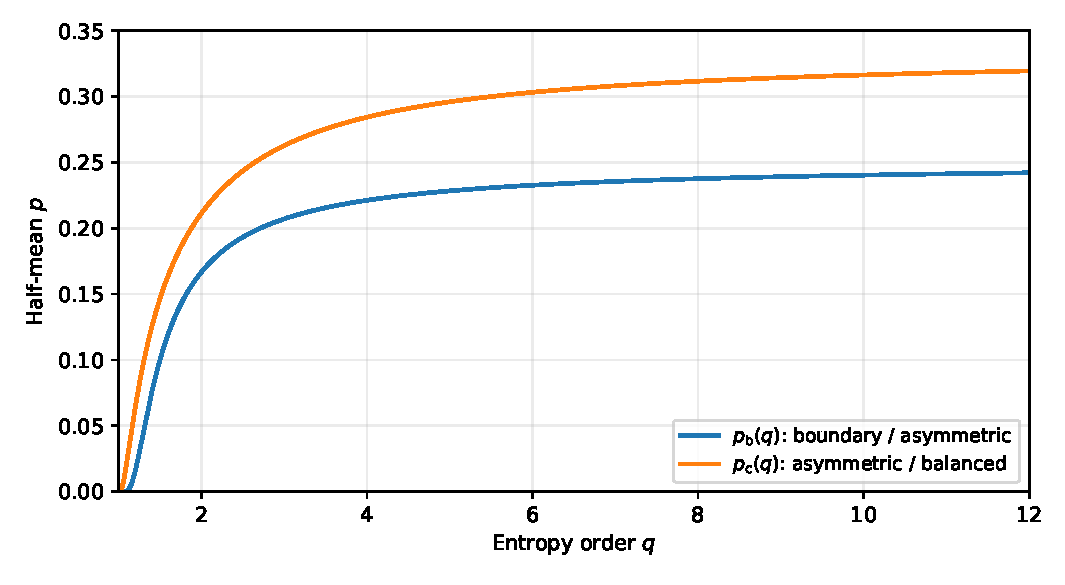
\includegraphics[width=.91\textwidth]{figures/phase_boundaries.pdf}
\caption{The exact boundaries \eqref{eq:pb} and \eqref{eq:pc}, plotted
numerically. Below the lower curve the optimizer is a boundary pair; between
the curves it is an unequal interior pair; above the upper curve it is the
balanced pair. The half-mean is $p=(p_1+p_2)/2\leq1/2$. The plot illustrates
Theorem~\ref{thm:phases}; it is not used in its proof.}
\label{fig:phases}
\end{figure}

The intermediate regime is important. Failure of concavity does not mean
that the best distribution must always have a deterministic summand.
There is an entire interval of means for which the unique unordered
maximizer consists of two distinct, strictly interior Bernoulli parameters.

\subsection{Closed formulas at order two}
Let $s=p_1+p_2$ and $r=p_1p_2$. The probability vector is
$(1-s+r,s-2r,r)$, so direct expansion gives
\begin{align}
 F_2(s,r)&=1-2s+2s^2+(2-6s)r+6r^2\label{eq:collisionpolynomial}\\
 &=6\left(r-\frac{3s-1}{6}\right)^2
   +\frac{5-6s+3s^2}{6}.\label{eq:completed}
\end{align}
For $0\leq s\leq1$, the feasible product interval is $0\leq r\leq s^2/4$.
Thus the exact optimizer is
\begin{equation}
 r_* = \max\left\{0,\min\left\{\frac{s^2}{4},\frac{3s-1}{6}\right\}\right\}.
 \label{eq:clamp}
\end{equation}
This gives the boundary regime $s\leq1/3$, the unequal interior regime
\[
 \frac13<s<1-\frac1{\sqrt3},
\]
and the balanced regime above it. In the middle regime,
\begin{equation}
 (p_1,p_2)=\frac12\left(s\pm\sqrt{s^2-2s+\frac23},\quad
                            s\mp\sqrt{s^2-2s+\frac23}\right),
 \label{eq:q2optimizer}
\end{equation}
and the minimum collision probability equals
$(5-6s+3s^2)/6$. The notation in \eqref{eq:q2optimizer} means the two
opposite sign choices, which exchange the coordinates.

On the path \eqref{eq:path}, the complete collision identity is
\begin{equation}
 F_2(p+t,p-t)-F_2(p,p)
 =-2(1-6p+6p^2)t^2+6t^4.\label{eq:q2path}
\end{equation}
It supplies a second way to check the rational certificate:
$p=1/10$ and $t=1/20$ give $F_2(p,p)-F_2(p+t,p-t)=181/80000$.

\begin{figure}[tbp]
\centering
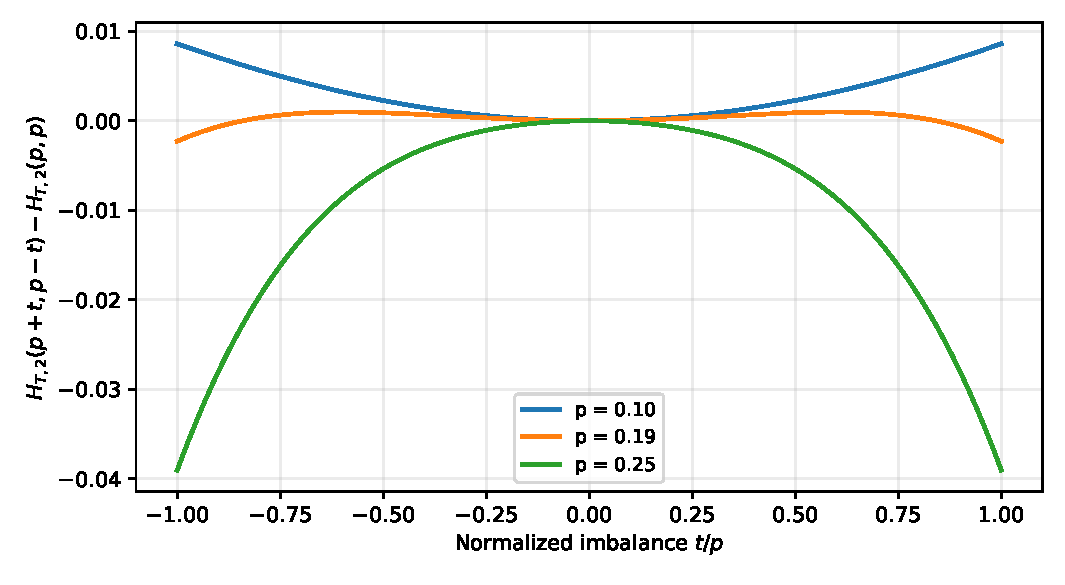
\includegraphics[width=.91\textwidth]{figures/collision_profiles.pdf}
\caption{Exact order-two Tsallis entropy differences from the balanced
value, evaluated from \eqref{eq:q2path}. The three half-means lie in the
boundary, unequal-interior and balanced regimes, respectively. A positive
value away from zero is a strict midpoint obstruction when the two symmetric
parameter points are used as endpoints.}
\label{fig:profiles}
\end{figure}

\section{The Shannon transition and subcritical fixed-mean concavity}
\subsection{Monotonicity and asymptotics of the boundaries}
\begin{proposition}\label{prop:asymptotics}
Both $\pb(q)$ and $\pc(q)$ are strictly increasing for $q>1$. With
$a=q-1$ and $L=\log2$, as $a\downarrow0$,
\begin{align}
 \pb(1+a)&=\frac12e^{-L/a}\bigl(1+O(e^{-L/a})\bigr),\label{eq:smallpb}\\
 \pc(1+a)&=\exp\left(-\sqrt{\frac{2L}{a}}+O(\sqrt a)\right).
 \label{eq:smallpc}
\end{align}
As $a\to\infty$,
\begin{equation}
 \pb(1+a)=\frac14-\frac{L}{8a}+O(a^{-2}),\qquad
 \pc(1+a)=\frac13-\frac{2L}{9a}+O(a^{-2}).\label{eq:largepq}
\end{equation}
\end{proposition}
\begin{proof}
Monotonicity of $\pb$ follows directly from \eqref{eq:pb}. Set
$g(a)=\arcosh(e^{La})$, with $g(0)=0$. For $a>0$,
\[
 g'(a)=\frac{L}{\sqrt{1-e^{-2La}}},\qquad
 g''(a)=-\frac{L^2e^{-2La}}{(1-e^{-2La})^{3/2}}<0.
\]
Strict concavity and $g(0)=0$ imply that $g(a)/a$ strictly decreases.
Equation~\eqref{eq:pc} then makes $\pc$ strictly increasing.
For small $a$, the expansion $\cosh z=1+z^2/2+O(z^4)$ gives
$g(a)=\sqrt{2La}\,(1+O(a))$. Substitution into \eqref{eq:pc} gives
\eqref{eq:smallpc}, while \eqref{eq:smallpb} is immediate.
For large $a$,
\[
 g(a)=(a+1)L+O(2^{-2a}).
\]
Expanding the two explicit boundary formulas in $1/a$ gives
\eqref{eq:largepq}.
\end{proof}

\begin{table}[tbp]
\centering
\begin{tabular}{@{}rrr@{}}
\toprule
$q$ & $p_{\mathrm{b}}(q)$ & $p_{\mathrm{c}}(q)$ \\
\midrule
1.01 & $3.944305\times10^{-31}$ & $7.597324\times10^{-6}$ \\
1.05 & $4.768367\times10^{-7}$ & 0.004986586 \\
1.1 & 0.000487805 & 0.022610828 \\
1.25 & 0.029411765 & 0.081406962 \\
1.5 & 0.100000000 & 0.146446609 \\
2 & 0.166666667 & 0.211324865 \\
3 & 0.207106781 & 0.262751066 \\
4 & 0.221246667 & 0.284370123 \\
10 & 0.240377712 & 0.316443755 \\
100 & 0.249124818 & 0.331779267 \\
\bottomrule
\end{tabular}

\caption{Numerical boundary values from the exact formulas; the CSV in the
archive retains more digits. For $q=1.01$ the balanced-point instability
requires a half-mean below about $7.6\times10^{-6}$, whereas the simple
boundary-optimizer condition is far more restrictive.}
\label{tab:boundaries}
\end{table}

The distinction between the two exponentially small scales is substantial.
The explicit dyadic construction guarantees a finite witness without solving
an equation, but is not close to the sharp local scale when $q$ is near one.
A coarse scan of moderate probabilities can therefore miss the instability
near Shannon entropy. This is an explanation of the sampling issue, not a
claim about how the original conjecture was tested.

\subsection{A nonuniform limit of curvature}
For any fixed $p\in(0,1/2]$, expansion of \eqref{eq:D} around $a=0$ gives
\begin{equation}
 D_{1+a}(p)=-2a\log2+O_p(a^2).\label{eq:Dnearone}
\end{equation}
Indeed the coefficient of $a$ is
$2\log(1-p)-2\log(2p(1-p))+2\log p=-2\log2$.
Consequently each of \eqref{eq:Tcurvature} and \eqref{eq:Rcurvature}
approaches $-4\log2$ as $q\downarrow1$.

In contrast, if $q>1$ is fixed and $p\downarrow0$, then $D_q(p)\to1$ and
$F_q(p,p)\to1$, so both curvatures approach
\begin{equation}
 \frac{2q}{q-1}>0.\label{eq:cornerlimit}
\end{equation}
Thus convergence to the Shannon curvature is not uniform near the
parameter boundary. There is no contradiction between the Shannon theorem
and counterexamples at every order immediately above one.

\subsection{A positive result below and at one}
Although general joint concavity for $0<q<1$ is not established here,
the fixed-mean two-coin problem admits a complete result.

\begin{theorem}[Concavity on every two-coin fixed-mean segment]
\label{thm:subcritical}
For each $0<q\leq1$ and each mean $s\in(0,2)$, R\'enyi and Tsallis entropy
are strictly concave along the nondegenerate interior of the two-coin
parameter segment $p_1+p_2=s$, using their common Shannon value at $q=1$.
They extend as concave functions to the closed segment. Their unique
maximizer is the balanced pair $(s/2,s/2)$.
\end{theorem}
\begin{proof}
By complement symmetry assume $s\leq1$ and use $p=s/2$, $u=t^2$.
First suppose $0<q<1$, so $a=q-1\in(-1,0)$. The factorization
\eqref{eq:Dfactor} is still valid at $u=0$. Since $2^a<1$,
\[
 y^2-2^{a+1}y+1=(y-2^a)^2+1-2^{2a}>0.
\]
Thus $D_q(p)>0$ and $G'(0)=-qD_q(p)<0$.
Equation~\eqref{eq:convexu} now has a negative prefactor $q(q-1)$, so
$G''(u)<0$ throughout the interior. Hence $G'(u)<0$ there. With
$K(t)=G(t^2)$, the chain rule gives
\begin{equation}
 K''(t)=2G'(t^2)+4t^2G''(t^2)<0.\label{eq:subcriticalchain}
\end{equation}
Tsallis entropy is $(K-1)/(1-q)$, so it is strictly concave. R\'enyi entropy
is $(\log K)/(1-q)$, and
$(\log K)''=K''/K-(K'/K)^2<0$, giving the same conclusion.
Evenness and strict decrease of $G$ in $u$ make $t=0$ the unique maximum.
Continuity of $x^q$ at zero extends concavity to the closed segment.

For $q=1$, write $J(u)=-\sum_{k=0}^2 f_k(u)\log f_k(u)$, with $f_k$ as in
\eqref{eq:G}. Direct differentiation gives
\begin{align}
 J'(u)&=\log\frac{f_0(u)f_2(u)}{f_1(u)^2},\label{eq:shannonderivative}\\
 J''(u)&=-\frac1{f_0(u)}-\frac4{f_1(u)}-\frac1{f_2(u)}<0.
\end{align}
For any two Bernoulli parameters $v,w$, the identity
$f_1=v(1-w)+w(1-v)$ and the arithmetic--geometric mean inequality imply
$f_1^2\geq4f_0f_2$. Thus $J'(u)\leq-\log4<0$.
Applying the chain rule as in \eqref{eq:subcriticalchain} proves strict
concavity in $t$, and continuity of $x\log x$ at zero handles the endpoints.
At $t=0$, $f_1^2=4f_0f_2$, so the second derivative is exactly $-4\log2$.
\end{proof}

This theorem concerns a one-dimensional family of directions in a
\emph{two}-dimensional parameter cube. It is not a proof of joint concavity
on that cube for $q<1$, much less for arbitrary numbers of coins.

\section{Minimum dimension and separate coordinate concavity}
\subsection{Tsallis entropy remains concave in each coordinate}
\begin{proposition}\label{prop:separate}
For every $n$ and every finite $q>0$, Tsallis entropy of a Bernoulli sum is
concave in each parameter separately, with all other parameters fixed.
Nevertheless it fails joint concavity when $n=2$ and $q>1$.
\end{proposition}
\begin{proof}
Remove coin $i$, and let $g_k$ be the probability mass function of the
remaining sum, extended by zero outside its support. With $z=p_i$,
\[
 f_k(z)=(1-z)g_k+zg_{k-1},\qquad d_k=g_{k-1}-g_k.
\]
For $q\ne1$ and $0<z<1$, direct differentiation gives
\begin{equation}
 \frac{\mathrm d^2}{\mathrm dz^2}H_{\mathrm T,q}
 =-q\sum_k d_k^2 f_k(z)^{q-2}\leq0.\label{eq:separate}
\end{equation}
Indices at which both $g_k$ and $g_{k-1}$ vanish are omitted; their
contribution is identically zero. The formula for $q=1$ is
$-\sum_k d_k^2/f_k(z)\leq0$. Continuity extends the conclusion to $z=0,1$.
The failure of joint concavity is Theorem~\ref{thm:main}.
\end{proof}

In particular, one coin cannot be a Tsallis counterexample at any finite
positive order. The minimum number of coins needed for failure is exactly
two for every $q>1$. Formula~\eqref{eq:hessian} gives a tangible matrix
explanation: a symmetric matrix may have negative diagonal entries while
possessing a positive eigenvalue.

\subsection{The one-coin R\'enyi calculation}
\begin{proposition}[Minimum number of coins for R\'enyi failure]
\label{prop:minimalrenyi}
For $1<q\leq2$, R\'enyi entropy of one Bernoulli variable is concave, so the
minimum number of coins needed for a counterexample is two. For every
finite $q>2$, one coin already gives failure.
\end{proposition}
\begin{proof}
Put $a=q-1$, $b=1-z$, and $C(z)=z^q+b^q$. Then
\[
 H_{\mathrm R,q}''(z)
 =-\frac{C''(z)C(z)-C'(z)^2}{aC(z)^2}.
\]
For $0<a\leq1$, set $x=z/b>0$ and $w=\log x$. Expanding the numerator gives
\begin{align}
 C''C-(C')^2
 &=q b^{2a}N_a(x),\\
 N_a(x)&=a x^{a-1}(1+x^2)+2(a+1)x^a-x^{2a}-1\\
 &=2x^a\bigl[a\cosh w+(a+1)-\cosh(aw)\bigr].
\end{align}
Convexity of $\cosh$ gives
$\cosh(aw)\leq a\cosh w+(1-a)\cosh0$.
Hence $N_a(x)\geq4a x^a>0$, proving strict concavity in the interior.
Continuity gives concavity on $[0,1]$.

If $q>2$, as $z\downarrow0$ we have
$C\to1$, $C'\to-q$, and $C''\to q(q-1)$. Therefore
\[
 H_{\mathrm R,q}''(z)\longrightarrow\frac q{q-1}>0.
\]
This supplies a one-coin convex interval. Combining these facts with
Theorem~\ref{thm:main} proves the minimum-dimension statements.
\end{proof}

For example, at $q=2$ the one-coin identity simplifies to
\[
 H_{\mathrm R,2}''(z)
 =-\frac{8z(1-z)}{\bigl(z^2+(1-z)^2\bigr)^2}\leq0.
\]
The elementary one-coin obstruction above order two is consistent with the
source's original test family; the two-coin antisymmetric direction is what
forces the bound down to one.

\section{Higher dimensions and structural consequences}
\subsection{Strictly interior counterexamples with any number of coins}
Appending deterministic zero coins immediately transfers a two-coin
counterexample to every larger dimension. A stronger statement avoids
boundary parameters altogether.

\begin{theorem}[Instability at small binomial parameter vectors]
\label{thm:anyn}
Fix $n\geq2$ and a finite $q>1$. For all sufficiently small $p>0$, each
entropy has positive second variation at $(p,\ldots,p)$ in the direction
$(1,-1,0,\ldots,0)$. Consequently every dimension $n\geq2$ admits a strict
interior midpoint counterexample of this form.
\end{theorem}
\begin{proof}
Let $W\sim\Bin(n-2,p)$ be the background sum, independent of the first two
coins, and write $g_k=\mathbb P(W=k)$ with zero extension. Convolving
\eqref{eq:threeprob} with $g$ shows that
\begin{equation}
 f_k(t)=f_k(0)-t^2\bigl(g_k-2g_{k-1}+g_{k-2}\bigr),
 \label{eq:background}
\end{equation}
where $f(0)$ is the $\Bin(n,p)$ mass function. All first derivatives at zero
vanish. Thus the Tsallis second variation is
\begin{equation}
 \frac{2q}{q-1}\sum_{k=0}^n f_k(0)^{q-1}
              \bigl(g_k-2g_{k-1}+g_{k-2}\bigr),\label{eq:anyncurv}
\end{equation}
and the R\'enyi second variation is this quantity divided by $F_q(0)>0$.
As $p\downarrow0$, the $k=0$ summand in \eqref{eq:anyncurv} tends to one.
For every $k\geq1$, $f_k(0)^{q-1}\to0$, while the bracket is bounded.
The finite sum therefore tends to one. Both second variations are positive
for sufficiently small $p$.
Choose $|t|$ sufficiently small compared with $p$. Smoothness gives a strict
local entropy minimum at $t=0$, and exchanging the first two coins makes
the two nonzero endpoints have equal entropy. All coordinates are interior.
\end{proof}

The proof is dimensionwise: the allowed size of $p$ may depend on $n$ and
$q$. No uniform-in-$n$ neighborhood is asserted.

\subsection{Parameter majorization and the geometry of the counterexample}
At a fixed small mean, averaging the two unequal parameter vectors in
Theorem~\ref{thm:dyadic} \emph{decreases} entropy. Thus neither entropy is
Schur-concave as a function of the Bernoulli \emph{parameters} for $q>1$.
Nor is it Schur-convex on the whole parameter square: at mean one,
Theorem~\ref{thm:curvature} shows that the balanced point $(1/2,1/2)$ is a
strict local maximum, reversing the required Schur-convex ordering.
These are statements about parameter vectors, not about majorization of
probability mass vectors.

There is an elementary distributional interpretation of the direction.
Increasing $u=t^2$ transfers mass $u$ from outcome zero and mass $u$ from
outcome two to outcome one. The mean stays fixed, while
\begin{equation}
 \Var(S)=2p(1-p)-2u
\end{equation}
decreases. When $p$ is small, the mass at zero is overwhelmingly the largest.
At orders above one, reducing that dominant mass can reduce the power sum
more than the loss of a rare outcome increases it. The resulting entropy
increase is therefore compatible with a decrease in variance. This
interpretation is encoded exactly, rather than assumed heuristically, in
\eqref{eq:Gprime}.

\subsection{What the result does not contradict}
The Shannon joint-concavity theorem is untouched. So are positive results
about monotone changes of one parameter, including the separate-coordinate
Tsallis inequality \eqref{eq:separate}. The later Hillion--Johnson question
about increasing parameters towards $1/2$ is a monotonicity question
\cite[Section~4]{HJ2019}; the present path has slopes of opposite signs and
is not a counterexample to that question. Likewise, convolution
entropy-power inequalities such as those studied in \cite{MMR2023} are not
Jensen inequalities in the Bernoulli parameters.

\section{Verification, computation and reproducibility}
\subsection{Three independent layers}
The mathematical argument is deliberately independent of a search program.
The main disproof consists of the three-probability identity
\eqref{eq:threeprob}, the derivative bound in
Lemma~\ref{lem:smallmean}, and the explicit arithmetic estimate in
Theorem~\ref{thm:dyadic}. The rational order-two certificate can be checked
without differentiation or logarithm evaluation.

The archive adds the following checks.
\begin{enumerate}[label=\textnormal{(\arabic*)}]
\item \texttt{code/verify\_exact.py} uses only Python's standard library and
exact rational arithmetic. The recorded run passed \textbf{12,512 checks}:
24 probability calculations were compared with independent exhaustive
outcome enumeration; the collision polynomial was tested on 441 rational
parameter pairs; 1,991 integer-order Jensen examples, 16 rational-order
sufficient-condition certificates, 11 higher-dimensional witnesses, and
9,999 fixed-mean optimizer comparisons were checked. The remaining checks
cover normalization and the main explicit certificate.
\item \texttt{code/verify\_symbolic.py} independently differentiates symbolic
expressions using SymPy. It checks the general center-curvature and quartic
identities, the collision polynomial, the one-coin order-two formula and
the exact Hessian \eqref{eq:hessian}.
\item \texttt{code/make\_figures.py} evaluates the explicit boundaries at
80-decimal working precision and produces the numerical CSV and vector
figures. These numerical illustrations play no role in the proof.
\end{enumerate}

A floating-point Hessian search was used during exploration to find promising
directions. Its script and log are retained for provenance, but no theorem
relies on an eigenvalue returned by floating-point linear algebra. In
particular, the exploratory log is not an exact certificate.

\subsection{Rebuilding}
From the archive's top-level directory, run
\begin{verbatim}
python code/verify_exact.py
python code/verify_symbolic.py
python code/make_figures.py
pdflatex -interaction=nonstopmode -halt-on-error article.tex
pdflatex -interaction=nonstopmode -halt-on-error article.tex
\end{verbatim}
Only the last two optional verification/illustration programs require
third-party Python libraries; the exact certificate checker has none.
A prebuilt PDF, the numerical table and the two figure PDFs are included,
so rebuilding the article itself does not require running Python.
The dependency versions used are recorded in \texttt{results/environment.txt}.

\section{Conclusions and remaining questions}
The proposed numerical generalized Shepp--Olkin thresholds are false in the
unrestricted affine-interpolation setting. The failure is already visible
with two independent coins, at a fixed mean, away from every face of the
parameter square. It persists for every finite order above one and defeats
even quasiconcavity. A single strict rational inequality at order two is
sufficient to disprove both proposed values.

The counterexample is not merely isolated. Its sharp curvature boundary is
\eqref{eq:pc}; its fixed-mean maximizers undergo the three rigorously
classified regimes of Theorem~\ref{thm:phases}; and its approach to the
Shannon order has the singular scale \eqref{eq:smallpc}. Below one,
Theorem~\ref{thm:subcritical} gives a positive result on every two-coin
fixed-mean segment, but not on every affine direction.

The most immediate remaining mathematical question is whether universal
joint concavity holds for all $0<q<1$. An affirmative result would complete
a corrected finite-order threshold theorem with threshold one. A second,
distinct question is what happens after restricting all interpolation
slopes to the same sign. The present construction deliberately uses a
mixed-sign direction and does not settle that restriction. A third is to
classify fixed-mean entropy maximizers for three or more Bernoulli
parameters; Theorem~\ref{thm:anyn} rules out a universal balanced-maximizer
principle above one, but is not such a classification.

\paragraph{Scope of the order parameter.}
All threshold and minimum-dimension assertions in this article concern
finite positive orders. In particular, the direct limit of the Tsallis
functional as $q\to\infty$ is the constant zero functional, since
$0\leq H_{\mathrm T,q}\leq1/(q-1)$. That limiting functional should not be
silently included in a finite-order threshold statement. No classification
at order zero is asserted here.

\paragraph{Research status.}
The article presents self-contained proofs, not just computational
suggestions, but it is an AI-assisted research draft. No independent referee
report, author confirmation, or proof-assistant verification is claimed.
The novelty claim is limited to what the documented literature search
established. These limitations concern review and priority; they do not
replace or weaken the explicit mathematical statements and proofs.

\appendix
\section{Random area selection and manifest exclusion}
The area list was fixed before a single call to Python's
\texttt{secrets.randbelow(96)}. The returned zero-based index was $57$, hence
the selected one-based area was $58$: \emph{Discrete probability}.
The original draw is in \texttt{notes/selection.json}; its full generating
script is in \texttt{code/select\_area.py}. There was no redraw.
Re-executing that script makes a \emph{new} random draw; it does not reproduce
the original OS randomness. The preserved JSON is the historical selection
record. The area labels overlap, so uniformity is over this declared list
of labels, not over an intrinsic partition of all mathematics.

The supplied \texttt{manifest(1).tex}, dated 20 September 2026, catalogues
71 research packages. All entries were read as exclusion targets, without
attempting to revalidate their claimed proofs. None concerns the numerical
R\'enyi/Tsallis thresholds, the two-coin fixed-mean problem, or the particular
Hillion--Johnson conjecture selected here. The exclusion audit is recorded
in \texttt{notes/manifest\_exclusion.md}.

\subsection*{The complete 96-area list}
\begin{multicols}{3}
\small
\begin{enumerate}[leftmargin=2.1em,label=\arabic*.,itemsep=.12em,parsep=0pt]
\item Additive combinatorics
\item Analytic number theory
\item Algebraic number theory
\item Diophantine approximation
\item Finite fields
\item Arithmetic dynamics
\item Combinatorial number theory
\item Integer partitions
\item Permutation patterns
\item Algebraic combinatorics
\item Enumerative combinatorics
\item Extremal set theory
\item Ramsey theory
\item Spectral graph theory
\item Structural graph theory
\item Graph polynomials
\item Graph labeling
\item Design theory
\item Coding theory
\item Matroid theory
\item Combinatorial geometry
\item Discrete geometry
\item Convex geometry
\item Lattice polytopes
\item Tiling theory
\item Combinatorics on words
\item Automata theory
\item Formal language theory
\item Semigroup theory
\item Finite group theory
\item Infinite group theory
\item Combinatorial group theory
\item Ring theory
\item Commutative algebra
\item Noncommutative algebra
\item Representation theory
\item Lie algebras
\item Universal algebra
\item Lattice theory
\item Order theory
\item Category theory
\item Type theory
\item Proof theory
\item Computability theory
\item Model theory
\item Set-theoretic topology
\item General topology
\item Algebraic topology
\item Knot theory
\item Low-dimensional topology
\item Differential geometry
\item Metric geometry
\item Geometric group theory
\item Dynamical systems
\item Symbolic dynamics
\item Ergodic theory
\item Probability inequalities
\item Discrete probability
\item Random walks
\item Stochastic processes
\item Special functions
\item Orthogonal polynomials
\item Continued fractions
\item Asymptotic analysis
\item Complex analysis
\item Geometric function theory
\item Harmonic analysis
\item Functional analysis
\item Banach space geometry
\item Operator theory
\item Matrix inequalities
\item Tensor algebra
\item Optimization theory
\item Discrete optimization
\item Numerical analysis
\item Approximation theory
\item Combinatorial game theory
\item Mathematical logic of games
\item Information theory
\item Boolean functions
\item Hypergraph theory
\item Incidence geometry
\item Finite geometry
\item Topological combinatorics
\item Cluster algebras
\item Tropical geometry
\item Algebraic statistics
\item Combinatorial commutative algebra
\item Symmetric functions
\item q-series
\item Difference equations
\item Functional equations
\item Fractional calculus
\item Integral inequalities
\item Potential theory
\item Fractal geometry

\end{enumerate}
\end{multicols}

\section{A compact independent certificate}
The following Python fragment is a complete exact verification of the
order-two Jensen obstruction. It uses neither the derivative formulas nor
any third-party package.
\begin{verbatim}
from fractions import Fraction as Q

def collision(a, b):
    f = ((1-a)*(1-b), a+b-2*a*b, a*b)
    return sum(x*x for x in f)

center = collision(Q(1,10), Q(1,10))
endpoint = collision(Q(3,20), Q(1,20))
assert center == Q(55088,80000)
assert endpoint == Q(54907,80000)
assert center - endpoint == Q(181,80000) > 0
\end{verbatim}
Both endpoint entropies are equal by exchanging the coins. For Tsallis
order two, subtracting the power sum from one reverses the displayed
inequality. For R\'enyi order two, applying the decreasing function
$-\log$ reverses it. Thus the fragment certifies a genuine Jensen failure,
not just a numerical approximation to one.

\begin{thebibliography}{9}
\bibitem{HJ2017}
E.~Hillion and O.~Johnson,
\emph{A proof of the Shepp--Olkin entropy concavity conjecture},
Bernoulli \textbf{23}(4B) (2017), 3638--3649.
\href{https://doi.org/10.3150/16-BEJ860}{doi:10.3150/16-BEJ860}.
Original version: \href{https://arxiv.org/abs/1503.01570}{arXiv:1503.01570v1}
(5 March 2015), especially Section~4 and Conjecture~4.2 on PDF page~7.

\bibitem{J2017}
O.~Johnson,
\emph{Entropy and thinning of discrete random variables},
The IMA Volumes in Mathematics and its Applications \textbf{161} (2017),
33--53.
\href{https://arxiv.org/abs/1510.05390}{arXiv:1510.05390v3}
(7 June 2016), Section~8, item~5.

\bibitem{HJ2019}
E.~Hillion and O.~Johnson,
\emph{A proof of the Shepp--Olkin entropy monotonicity conjecture},
Electronic Journal of Probability \textbf{24} (2019), paper~126, 1--14.
\href{https://arxiv.org/abs/1810.09791}{arXiv:1810.09791}.
The R\'enyi and Tsallis monotonicity discussion is in Section~4.

\bibitem{MMR2023}
M.~Madiman, J.~Melbourne and C.~Roberto,
\emph{Bernoulli sums and R\'enyi entropy inequalities},
Bernoulli \textbf{29}(2) (2023), 1578--1599.
\href{https://doi.org/10.3150/22-BEJ1511}{doi:10.3150/22-BEJ1511}.
\href{https://arxiv.org/abs/2103.00896}{arXiv:2103.00896}; the version consulted
was v2, dated 15 March 2024.
\end{thebibliography}
\end{document}
